%%% UNIT 5
{
\setbeamertemplate{headline}{}
\setbeamertemplate{footline}{
  \begin{beamercolorbox}[wd=\paperwidth,ht=2.2ex,dp=1.5ex]{palette quaternary}
  \end{beamercolorbox}
  }
\begin{frame}[noframenumbering]
\frametitle{\DB{\huge{\textbf{$\blacksquare$ Unit 5}}}}
\myPause
 \begin{itemize}
 \item[] \LARGE{\MB{Practice session 2 --- with some theory embedded}}
 \item[] \vspace{-1mm}\hspace{5mm}\Large{\MB{System responses (just a bit)}}
 \item[] \vspace{-1mm}\hspace{5mm}\Large{\MB{Direct synthesis}}
 \item[] \vspace{-1mm}\hspace{5mm}\Large{\MB{PI (D to come) for the man in the road}}
 \item[] \vspace{-1mm}\hspace{5mm}\Large{\MB{PI in the class}}
 \end{itemize}
\end{frame}
}

\part{}

\section{Foreword}
\subsection{}

\begin{frame}
\frametitleTC{Direct synthesis -- choosing $G_{yw}^{\circ}$ and $G_{yd}^{\circ}$}
\framesubtitleTC{The ideal selection}
\myPause
 \begin{center}
  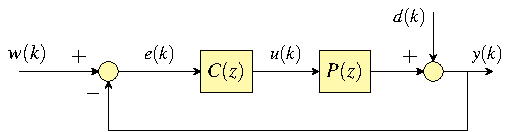
\includegraphics[width=0.50\columnwidth]{./Unit-04/img/ControlLoop-H1.pdf}
 \end{center}\myPause
 \begin{itemize}[<+-| alert@+>]
 \item If possible, we would like to have
       \begin{displaymath}
        G_{yw}^{\circ}(z) = \frac{1-\alpha}{z-\alpha}, \quad
        G_{yd}^{\circ}(z) = \frac{z-1}{z-\alpha}, \qquad
        0 < \alpha < 1.
       \end{displaymath}
 \item The reason is that this gives the best tracking of a step set point\\
       variation, and the best rejection of a step disturbance. 
 \end{itemize}
\end{frame}

\begin{frame}[fragile]
\frametitleTC{Direct synthesis -- choosing $G_{yw}^{\circ}$ and $G_{yd}^{\circ}$}
\framesubtitleTC{The ideal selection}
\myPause
 \begin{itemize}[<+-| alert@+>]
 \item What do we mean ``best''?
 \item Try in Scilab some values of $\alpha$, say 0.1, 0.5 and 0.9, and plot the corresponding\\
       step responses:
       {\scriptsize
       \begin{verbatim}
     Gyw = syslin('d',(1-0.5)/(%z-0.5)); // Example with alpha=0.5
     Gyd = syslin('d',(%z-1)/(%z-0.5));
     wd  = ones(1,20);                   // Step inputs (w for Gyw, d for Gyd)
     yw  = dsimul(tf2ss(Gyw),wd); 
     yd  = dsimul(tf2ss(Gyd),wd); 
     plot(yw,'b');                       // Response of Gyw in blue
     plot(yd,'r');                       // Response of Gyd in red
       \end{verbatim}
       }
 \item \vspace{-4mm}Comments:
       \begin{itemize}[<+-| alert@+>]
       \item exact asymptotic tracking of $w$, no overshoot, no oscillations;
       \item exact asymptotic rejection of $d$, monotonic response;
       \item the one parameter $\alpha$ governs tracking/rejection speed, namely\\
             $\alpha\rightarrow 0 \Rightarrow$ faster (\TC{``fast pole''}),\\
             $\alpha\rightarrow 1 \Rightarrow$ slower (\TC{``slow pole''}).
       \end{itemize}
 \item Are there alternatives? Yes --- come to advanced control courses \smiley.
 \end{itemize}
\end{frame}

\section{Exercise 01}
\subsection{}

\begin{frame}
\frametitleTC{Direct synthesis for set point tracking}
\framesubtitleTC{Some examples}
\myPause
 \begin{itemize}[<+-| alert@+>]
 \item Example 1 (OK):
       \begin{displaymath}
        \begin{array}{lcl}
         P(z)              = \frac{(z-0.5)}{(z-0.4)^2},\,
         G_{yw}^{\circ}(z) = \frac{0.2}{z-0.8} &
         \Rightarrow &
         C(z)              = \frac{0.2(z-0.4)^2}{(z-1)(z-0.5)}.
        \end{array}
       \end{displaymath}
 \item Example 2 (\red{NO}, process pole outside the circle $\Rightarrow$ unstable hidden part):
       \begin{displaymath}
        \begin{array}{lcl}
         P(z)              = \frac{1}{\red{z-2}},\,
         G_{yw}^{\circ}(z) = \frac{0.2}{z-0.8} &
         \Rightarrow &
         C(z)              = \frac{0.2\red{(z-2)}}{z-1}.
        \end{array}
       \end{displaymath}
 \item Example 3 (\red{NO}, infeasible relative degree):
       \begin{displaymath}
        \begin{array}{lcl}
         P(z)              = \frac{1}{(z-0.4)^2},\,
         G_{yw}^{\circ}(z) = \frac{0.2}{z-0.8} &
         \Rightarrow &
         C(z)              = \frac{0.2(z-0.4)^{\textcolor{red}{2}}}{z-1}.
        \end{array}
       \end{displaymath}
 \item Try one/two cases of your own, verify that everything is clear,\\
       ask questions if necessary.
 \end{itemize}
\end{frame}

\begin{frame}
\frametitleTC{Direct synthesis for set point tracking}
\framesubtitleTC{Dealing with the limitations}
\myPause
 \begin{itemize}[<+-| alert@+>]
 \item If the process has poles on or outside the circle, we must preserve them in the desired loop transfer
       function
       \begin{displaymath}
        L^{\circ}(z) = \frac{G_{yw}^{\circ}(z)}{1-G_{yw}^{\circ}(z)}
       \end{displaymath}
       so as to not have $C(z)$ cancel them and generate an unstable hidden part.
 \item If the process has zeroes on or outside the circle, we must include them in $G_{yw}^{\circ}(z)$\\
       -- hence in $L^{\circ}(z)$ -- so that $C(z)$ does not cancel them either; this may\\
       require to also add poles to have at least as many as there are zeroes.
 \item If the relative degree of $G_{yw}^{\circ}(z)$ is infeasible, we need to add ``fast''\\
       (near to the origin) poles and/or delay terms.
 \item\vfill Let us clarify with a few simulation examples. 
 \end{itemize}
\end{frame}


\begin{frame}[fragile]
\frametitleTC{Direct synthesis for set point tracking}
\framesubtitleTC{Dealing with the limitations -- Scilab script (1/3, copy{\&}paste to try at home)}
{\tiny
\def\baselinestretch{0.3}
\begin{verbatim}
// Direct synthesis examples -- set point tracking
clear; clc; z = %z;
// Reference and time vectors
w  = ones(1,30); 
k  = 0:length(w)-1;
// Process 1, asymptotically stable, no zeroes
P1 = syslin('d',2/(z-0.5)^2);
// Infeasible relative degree
To = syslin('d',0.2/(z-0.8));
R  = 1/P1*To/(1-To); disp(R); y1 = dsimul(tf2ss(To),w);
// Adding a fast pole for a realisable R
To = syslin('d',0.16/(z-0.8)/(z-0.2));
R  = 1/P1*To/(1-To); disp(R); y2 = dsimul(tf2ss(To),w);
// Adding a faster pole
To = syslin('d',0.19/(z-0.8)/(z-0.05));
R  = 1/P1*To/(1-To); disp(R); y3 = dsimul(tf2ss(To),w);
// Adding a one-step delay
To = syslin('d',0.2/(z-0.8)/z);
R  = 1/P1*To/(1-To); disp(R); y4 = dsimul(tf2ss(To),w);
// Using two poles, both faster than the design one
p1 = 0.75;
p2 = 0.45;
To = syslin('d',(1-p1)*(1-p2)/(z-p1)/(z-p2));
R  = 1/P1*To/(1-To); disp(R); y5 = dsimul(tf2ss(To),w);
\end{verbatim}
}
\end{frame}

\begin{frame}[fragile]
\frametitleTC{Direct synthesis for set point tracking}
\framesubtitleTC{Dealing with the limitations -- Scilab script (2/3)}
{\tiny
\def\baselinestretch{0.3}
\begin{verbatim}
// Process 2, asymptotically stable,, 1 zero outside the circle
P2 = syslin('d',(z-2)/(z-0.5)^2);
// Infeasible To
To = syslin('d',0.2/(z-0.8));
R  = 1/P2*To/(1-To); disp(R); y6 = dsimul(tf2ss(To),w);
// Adding the required zero to To
To = syslin('d',-0.18*(z-2)/(z-0.8)/(z-0.1));
R  = 1/P2*To/(1-To); disp(R); y7 = dsimul(tf2ss(To),w);
// Improving by acting on the To poles
p1 = 0.78;
p2 = 0.02;
To = syslin('d',-(1-p1)*(1-p2)*(z-2)/(z-p1)/(z-p2));
R  = 1/P2*To/(1-To); disp(R);
y8 = dsimul(tf2ss(To),w);
\end{verbatim}
}
\end{frame}

\begin{frame}[fragile]
\frametitleTC{Direct synthesis for set point tracking}
\framesubtitleTC{Dealing with the limitations -- Scilab script (3/3)}
{\tiny
\def\baselinestretch{0.3}
\begin{verbatim}
// Plot the results for process 1
h               = scf(0); clf;
h.figure_size   = [500,500];
title("${\Large \text{Cases 1--5}$");
xlabel("k");
plot(k,y1,'r',k,y1,'r.');
plot(k,y2,'b',k,y2,'b.');
plot(k,y3,'m',k,y3,'m.');
plot(k,y4,'g',k,y4,'g.');
plot(k,y5,'k',k,y5,'k.');
ax              = gca();
ax.data_bounds  = [0,0;max(k),1.1];
ax.tight_limits = "on";
// Plot the results for process 2
h               = scf(1); clf;
h.figure_size   = [500,500];
title("${\Large \text{Cases 6--8}$");
xlabel("k");
plot(k,y6,'r',k,y6,'r.');
plot(k,y7,'b',k,y7,'b.');
plot(k,y8,'k',k,y8,'k.');
ax              = gca();
ax.data_bounds  = [0,-0.3;max(k),1.1];
ax.tight_limits = "on";
\end{verbatim}
}
\end{frame}

\begin{frame}
\frametitleTC{Synthesis for set point tracking}
\framesubtitleTC{Dealing with the limitations -- summary}
\myPause
\begin{center}
 {\scriptsize
 \begin{tabular}{llll}
  \hline
Case & Process                   & Requirement                                                           & Controller  \\
\hline\hline
1& $P_1(z)=\frac{2}{(z-0.5)^2}$  & $G_{yw,11}^{\circ}(z)=\frac{0.2}{z-0.8}$                              & Infeasible  \\
2&                               & $G_{yw,12}^{\circ}(z)=\frac{0.16}{(z-0.8)(z-0.2)}$                    & $C_{12}(z)$ \\
3&                               & $G_{yw,13}^{\circ}(z)=\frac{0.19}{(z-0.8)(z-0.05)}$                   & $C_{13}(z)$ \\
4&                               & $G_{yw,14}^{\circ}(z)=\frac{0.2}{z(z-0.8)}$                           & $C_{14}(z)$ \\
5&                               & $G_{yw,15}^{\circ}(z)=\frac{(1-0.75)(1-0.45)}{(z-0.75)(z-0.45)}$      & $C_{15}(z)$ \\
\hline
6& $P_2(z)=\frac{z-2}{(z-0.5)^2}$& $G_{yw,21}^{\circ}(z)=\frac{0.2}{z-0.8}$                              & Infeasible  \\
7&                               & $G_{yw,22}^{\circ}(z)=-\frac{0.18(z-2)}{(z-0.8)(z-0.1)}$              & $C_{22}(z)$ \\
8&                               & $G_{yw,23}^{\circ}(z)=-\frac{(1-0.78)(1-0.02)(z-2)}{(z-0.78)(z-0.02)}$& $C_{23}(z)$ \\
  \hline
 \end{tabular}
 }
\end{center}
\end{frame}

\begin{frame}
\frametitleTC{Synthesis for set point tracking}
\framesubtitleTC{Dealing with the limitations -- results}
\myPause
\begin{center}
 {\scriptsize
 \begin{tabular}{ll}
  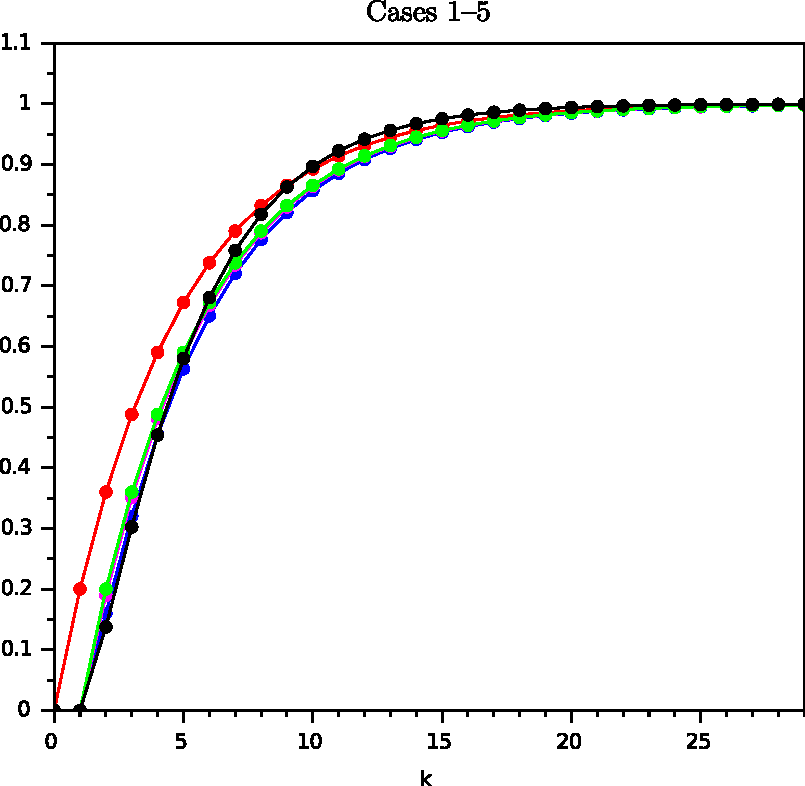
\includegraphics[width=0.35\textwidth]{./Unit-05/img/PS02-ex01-res-1to5.pdf} &
  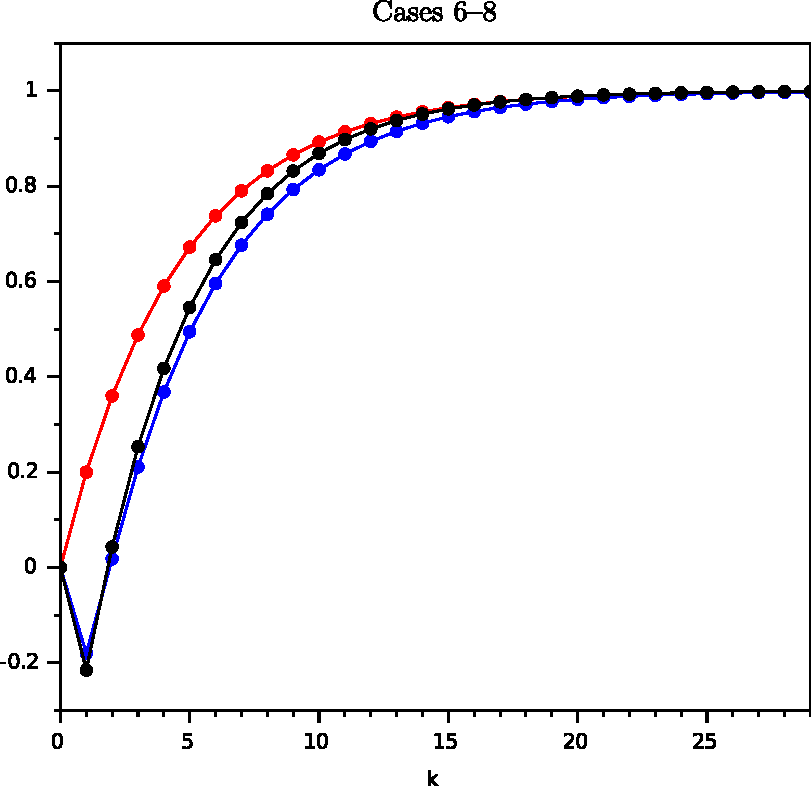
\includegraphics[width=0.35\textwidth]{./Unit-05/img/PS02-ex01-res-6to8.pdf}      \\
   \red{$P_1,G_{yw,11}^{\circ}\Rightarrow$ infeasible} &  \red{$P_2,G_{yw,21}^{\circ}\Rightarrow$ infeasible} \\
  \blue{$P_1,G_{yw,12}^{\circ}\Rightarrow$ $C_{12}$}   & \blue{$P_2,G_{yw,22}^{\circ}\Rightarrow$ $C_{22}$}   \\
   \mgt{$P_1,G_{yw,13}^{\circ}\Rightarrow$ $C_{13}$}   &       $P_2,G_{yw,23}^{\circ}\Rightarrow$ $C_{23}$    \\
   \grn{$P_1,G_{yw,14}^{\circ}\Rightarrow$ $C_{14}$}   \\
        $P_1,G_{yw,15}^{\circ}\Rightarrow$ $C_{15}$    \\
 \end{tabular}
 }
\end{center}
\end{frame}


\begin{frame}
\frametitleTC{Synthesis for set point tracking}
\framesubtitleTC{Summary}
\myPause
 \begin{itemize}[<+-| alert@+>]
 \item The technique is powerful, however there are \TC{objective} limits.
 \item In many of the cases seen the controller has one or two zeroes and one or two poles, 
       one of which in $z=1$.
 \item We shall soon call this a PI(D).
 \item \vfill You can try at home: open Scilab, launch the code editor SciNotes\\
       from the \texttt{Applications} menu, enter the code from the previous\\
       slides (copy{\&}paste) and run with the \texttt{Execute} command\\
       --- all IDEs look pretty much the same, in the end...
 \end{itemize}
\end{frame}

\section{Exercise 02}
\subsection{}

\begin{frame}
\frametitleTC{Building a block diagram in Modelica}
\framesubtitleTC{and experimenting with direct synthesis}
\myPause
 \begin{itemize}[<+-| alert@+>]
 \item Launch the model editor OMEdit.
 \item Issue \texttt{File->New Modelica Class}.
 \item Name the class \texttt{PID4CS}, select \texttt{Package} as \texttt{Specialization}. \underline{un}check\\
       \texttt{Save contents in one file} and click \texttt{OK.}
 \item You just created a \texttt{package}, a hierarchically organised collection\\
       of models.\\
 \item Right-click the P (Package) entry \texttt{PID4CS} in the \texttt{Libraries Browser}\\
       on the left, select \texttt{Save As}, and save. A folder named PID4CS\\
       will be created at the location you chose, details on its structure\\
       (inessential here) at \texttt{modelica.org} for the interested.
 \item Right-click \texttt{PID4CS} in the \texttt{Libraries Browser} and select\\
       \texttt{New Modelica Class}.
 \item Create a \texttt{Model} named \texttt{PS02\_ex02}, that will be part of \texttt{PID4CS}.\\
       Expand the entry (small triangle icon on the left) to see.
 \end{itemize}
\end{frame}

\begin{frame}
\frametitleTC{Building a block diagram in Modelica}
\framesubtitleTC{and experimenting with direct synthesis}
\myPause
 \begin{itemize}[<+-| alert@+>]
 \item No more details on the \texttt{Libraries Browser}, it works like any file manager.
 \item Double-click \texttt{PS02\_ex02} to edit: your window should look like
       \begin{center}
        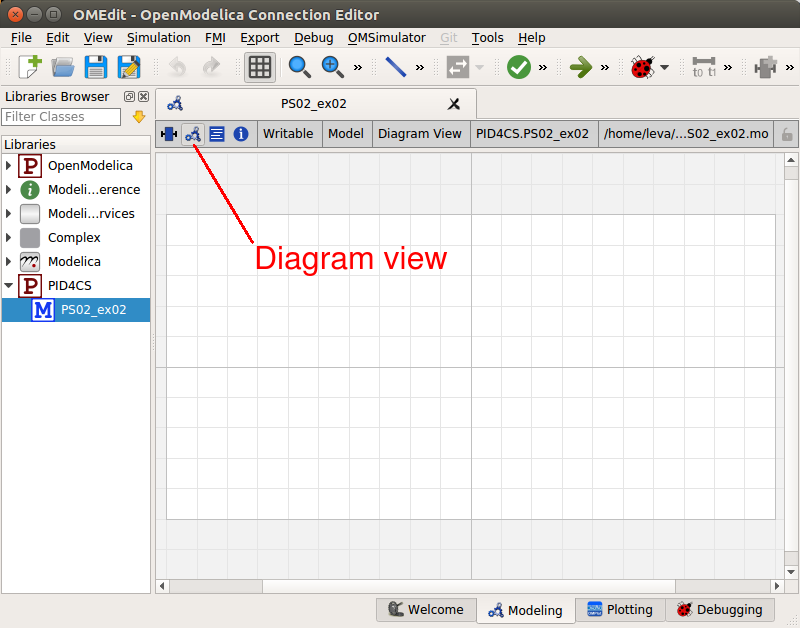
\includegraphics[width=0.40\columnwidth]{./Unit-05/img/PS02-ex02-fig01.png}
       \end{center}
       and you should be in \texttt{Diagram view} (click its button if not).
 \end{itemize}
\end{frame}

\begin{frame}
\frametitleTC{Building a block diagram in Modelica}
\framesubtitleTC{and experimenting with direct synthesis}
\myPause
 \begin{itemize}[<+-| alert@+>]
 \item Open the \texttt{Modelica Standard Library} (MSL for short); it is the \texttt{Modelica}
       entry in the \texttt{Libraries Browser}.
 \item Navigate to the \texttt{Blocks} package, that contains block diagram elements.
 \item You need \texttt{Transfer Function} from the \texttt{Discrete} sub-package, \texttt{Add}
       and \texttt{Feedback} from the \texttt{Math} one, and \texttt{RealExpression} from \texttt{Sources}.
 \item By dragging{\&}dropping from the browser, and wiring by click{\&}drag, create the\\
       diagram below (block types added for your reference, names above blocks):
       \begin{center}
        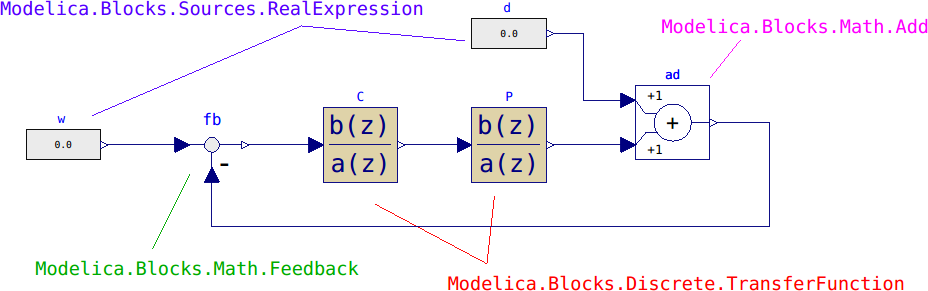
\includegraphics[width=0.60\columnwidth]{./Unit-05/img/PS02-ex02-fig02.png}
       \end{center}
 \end{itemize}
\end{frame}

\begin{frame}
\frametitleTC{Building a block diagram in Modelica}
\framesubtitleTC{and experimenting with direct synthesis}
\myPause
 \begin{itemize}[<+-| alert@+>]
 \item Double-click on the \texttt{P} and \texttt{C} blocks to set their transfer functions. Polynomials\\
       are specified as vectors of coefficient in decreasing power order: for example,\\
       $2z^3+z+5$ becomes \{2,0,1,5\}. Do not forget the braces and the zero entries\\
       for possibly missing powers --- including the constant term, $z$ becomes \{1,0\}.
 \item You also need to set a \texttt{samplePeriod}, i.e., the time between $k$ and $k+1$\\
       (in seconds). For this exercise it is inessential, enter 1 throughout.
 \item Double-click on the \texttt{w} and \texttt{d} blocks to enter the expression of their output\\
       as a function of time (the symbol \texttt{time} is system-declared).\\
       For example, $w=step(k)$ and $d=step(k-10)$ become respectively\\
       \texttt{if time<0 then 0 else 1} and \texttt{if time<10 then 0 else 1}.
 \end{itemize}
\end{frame}

\begin{frame}
\frametitleTC{Building a block diagram in Modelica}
\framesubtitleTC{and experimenting with direct synthesis}
\myPause
 \begin{itemize}[<+-| alert@+>]
 \item Issue \texttt{Simulation->Simulation Setup} to set the final time and then \texttt{Simulate}.
 \item Use the \texttt{Variable Browser} in the \texttt{Plotting} tab to examine the results. Below\\
       is an example with some explanatory lettering.
       \begin{center}
        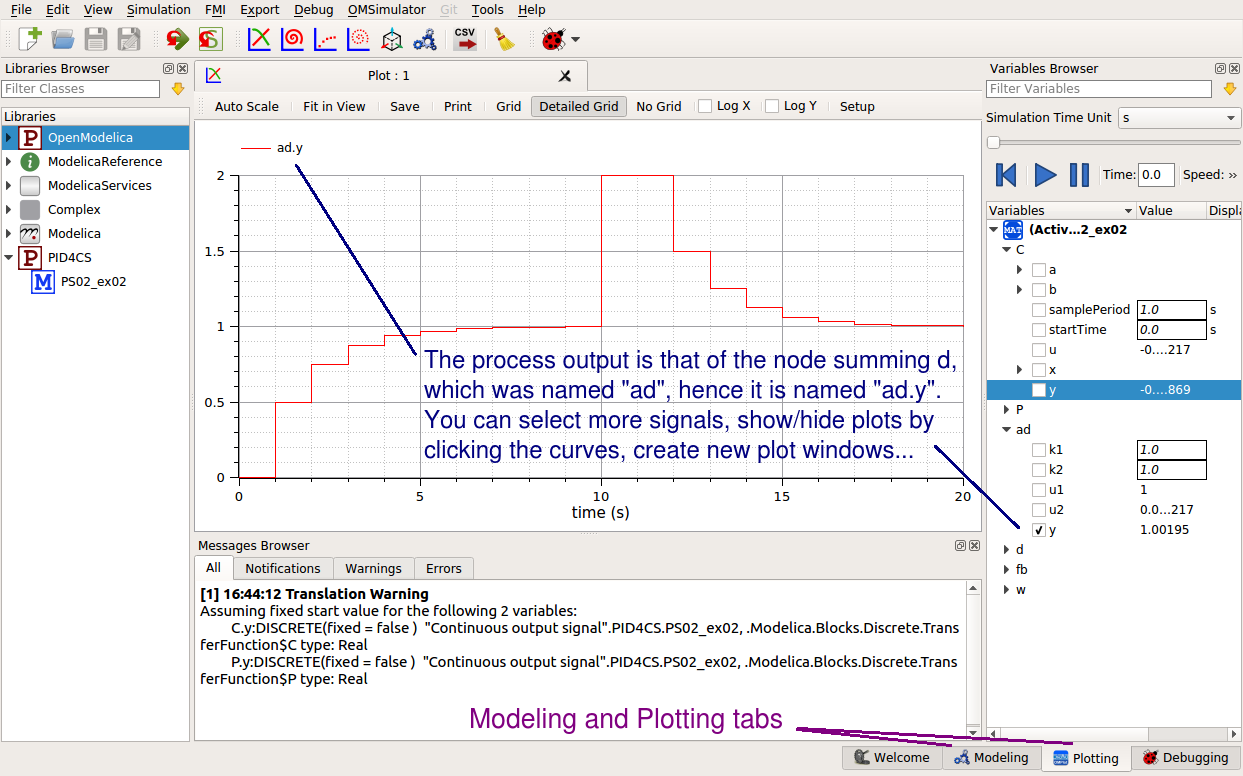
\includegraphics[width=0.60\columnwidth]{./Unit-05/img/PS02-ex02-fig03.png}
       \end{center}
 \end{itemize}
\end{frame}

\begin{frame}
\frametitleTC{Building a block diagram in Modelica}
\framesubtitleTC{and experimenting with direct synthesis}
\myPause
 \begin{itemize}[<+-| alert@+>]
 \item Please take some time at home to familiarise with OMEdit: it is quite intuitive\\
       and you can find plenty of tutorials online, many with videos. 
 \item For the moment, replicate for example the case with unstable hidden part:
       \begin{displaymath}
        \begin{array}{lcl}
         P(z)              = \frac{1}{\red{z-2}},\,
         G_{yw}^{\circ}(z) = \frac{0.2}{z-0.8} &
         \Rightarrow &
         C(z)              = \frac{0.2\red{(z-2)}}{z-1}.
        \end{array}
       \end{displaymath}
 \item Below is the plot of $y$ (\texttt{ad.y}) and $u$ (\texttt{C.y}) for $w=step(k)$ and $d=step(k-30)$.\\
       Apparently, something happens that $G_{yw}$ does not tell...
       \begin{center}
        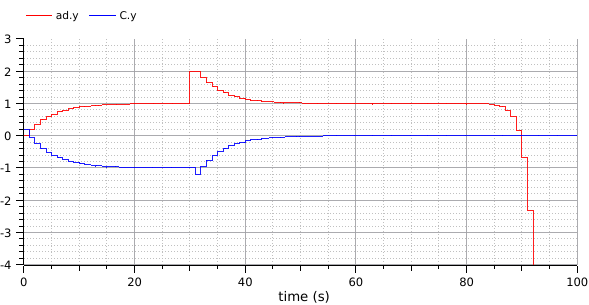
\includegraphics[width=0.50\columnwidth]{./Unit-05/img/PS02-ex02-fig04.png}
       \end{center}
 \end{itemize}
\end{frame}


\section{Exercise 03}
\subsection{}

\begin{frame}
\frametitleTC{Direct synthesis for disturbance rejection}
\framesubtitleTC{In fact, slightly more than a remark}
\myPause
 \begin{itemize}[<+-| alert@+>]
 \item The loop  and the closed-loop transfer functions are tied to one another: since
       \begin{displaymath}
        G_{yw}(z) = \frac{L(z)}{1+L(z)}, \qquad
        G_{yd}(z) = \frac{1}{1+L(z)},
       \end{displaymath}
 \item we have
       \begin{displaymath}
         L(z) = \frac{G_{yw}(z)}{1-G_{yw}(z)}, \quad
         L(z) = \frac{1-G_{yd}(z)}{G_{yd}(z)}, \quad
         G_{yw}(z)+G_{yd}(z) = 1.
       \end{displaymath}
 \item As a consequence,
       \begin{displaymath}
        G_{yw}(z) = \frac{1-\alpha}{z-\alpha} \quad \Rightarrow \quad
        G_{yd}(z) = 1-\frac{1-\alpha}{z-\alpha}
                  = \frac{z-1}{z-\alpha}
       \end{displaymath}
       and we are just back to the tracking problem.
 \end{itemize}
\end{frame}

\begin{frame}
\frametitleTC{Direct synthesis for disturbance rejection}
\framesubtitleTC{In fact, slightly more than a remark}
\myPause
 \begin{itemize}[<+-| alert@+>]
 \item We can revisit the previous exercise focusing on the disturbance response.
 \item In doing so, it is interesting to also look at the behaviour of the \TC{control signal}\\
       (in our Modelica diagram, \texttt{C.y}).
 \item Observe how a faster rejection -- like a faster tracking -- requires a larger peak\\
       in that signal (which is quite intuitive).
 \item As we shall see, this may lead to require something that the system -- or more\\
       precisely, the \TC{actuator} -- cannot do (e.g., allocate more cores than those\\
       aboard the machine).
 \item Incidentally, this means that \TC{architectures need sizing for fast enough\\
       reaction to TIME-VARYING \emph{stimuli}, not just for a worst-case\\
       CONSTANT load} --- hence one has to know about dynamics.
 \item \vfill Enough on this for the moment, please experiment at home \& report.
 \end{itemize}
\end{frame}

\section{PI for the man in the road}
\subsection{}

\begin{frame}
\frametitleTC{Foreword}
\framesubtitleTC{PI (Proportional plus Integral) control as an intuitive idea}
\myPause
 \begin{itemize}[<+-| alert@+>]
 \item We now introduce PI control in a totally intuitive manner, ie., the way\\
       ``the man in the road'' would do --- and incidentally, the way somebody\\
       says it was initially invented (we are not discussing this).
 \item The purpose of this part of our activity is twofold:
       \begin{itemize}[<+-| alert@+>]
       \item show that PI control is intuitive indeed,
       \item but also that intuition without theory is often misleading.    
       \end{itemize}
 \item Exercise: as we proceed, try to spot the flaws (not necessarily true ``errors''\\
       but symptoms of a partial viewpoint) in the reasoning by the man\\
       in the road and take note of them...
 \item[] \vspace{-0.75mm}...and then, when we re-visit the matter formally later on, check\\
       your notes to see if you spotted \underline{all} such flaws.
 \end{itemize}
\end{frame}

\begin{frame}
\frametitleTC{Intuition \# 1}
\framesubtitleTC{Proportional control}
\myPause
 \begin{itemize}[<+-| alert@+>]
 \item The man in the road says: \blue{``the farther the controlled variable $y$ is\\
       from the reference $w$, the more intense the control action $u$ has to be''}.
 \item \vfill Naming $e$ the error $w-y$, this introduces the \TC{Proportional (P) action}
       \begin{displaymath}
        u_P(k) = K_P \, e(k),
       \end{displaymath}
       where $K_P$ is a configuration parameter.
 \item Seems definitely a good idea.
 \item However $u_P$ is nonzero only if so is $e$, hence with P action alone
       \begin{itemize}[<+-| alert@+>]
       \item either $y$ can stay at ANY value ($w$ can be anything) with $u=0$,
       \item or one has to accept an error to have a control action.    
       \end{itemize} 
 \end{itemize}
\end{frame}

\begin{frame}
\frametitleTC{Intuition \# 2}
\framesubtitleTC{Introducing an automatic bias}
\myPause
 \begin{itemize}[<+-| alert@+>]
 \item Alternatively, a bias can be included in $u$ so as to zero the error:
       \begin{displaymath}
        u(k) = u_P(k)+ u_{bias}.
       \end{displaymath}
 \item But how to compute $u_{bias}$?
 \item The man in the road says: \blue{``automatically; if the error is zero keep it constant\\
       because you found the right value, otherwise increase or decrease it at each step,\\
       proportionally to the error''}.    
 \item This means
       \begin{displaymath}
        u_{bias}(k) = u_{bias}(k-1)+ K_{bias} e(k),
       \end{displaymath}
       where $K_{bias}$ is another configuration parameter.
 \end{itemize}
\end{frame}

\begin{frame}
\frametitleTC{Intuition \# 3}
\framesubtitleTC{Toward integral control}
\myPause
 \begin{itemize}[<+-| alert@+>]
 \item The main in the road continues: \blue{``the automatic bias is also consistent with the\\
       idea that if the error does not diminish this means that the system is reluctant\\
       to obey to the control action, hence the said action has to become stronger\\
       and stronger''}. 
 \item In fact, $u_{bias}(k)$ as just defined, sums each new error weighed by $K_{bias}$, which comes
       to determine the ratio of the control variation \TC{rate} to the value of the error.
 \item We can say that this is \TC{integrating} the error, and name the corresponding control component
       the \TC{Integral (I) action}
       \begin{displaymath}
        u_I(k) = u_I(k-1)+ K_I e(k),
       \end{displaymath}
        with $K_I$ as the second controller configuration parameter besides $K_P$.
 \end{itemize}
\end{frame}

\begin{frame}
\frametitleTC{The PI control law}
\framesubtitleTC{}
\myPause
 \begin{itemize}[<+-| alert@+>]
 \item The control signal is the sum of the P and the I action:
       \begin{displaymath}
        \left\{\begin{array}{rcl}
         u_P(k) &=& K_P \, e(k) \\
         u_I(k) &=& u_I(k-1)+ K_I e(k) \\
         u(k)   &=& u_P(k)+u_I(k)
        \end{array}\right.
       \end{displaymath}
 \item \vfill Intuition basically stops here.
 \item To understand how to give a value to $K_P$ and $K_I$ (or to the more\\
       comfortable equivalent parameters we shall define in the following)\\
       we must resort to theory.
 \end{itemize}
\end{frame}

\section{PI in the class}
\subsection{}

\begin{frame}
\frametitleTC{Transfer function}
\framesubtitleTC{}
\myPause
 \begin{itemize}[<+-| alert@+>]
 \item Let us reload our systems theory knowledge:
       \begin{displaymath}
        \left\{\begin{array}{rcl}
         u_P(k) &=& K_P \, e(k) \\
         u_I(k) &=& u_I(k-1)+ K_I e(k) \\
         u(k)   &=& u_P(k)+u_I(k)
        \end{array}\right. \quad
        {\Rightarrow} \quad
        \left\{\begin{array}{rcl}
         zu_I(k) &=& u_I(k) + zK_I e(k) \\
         u(k)    &=& u_I(k) + K_P \, e(k)
        \end{array}\right.
       \end{displaymath}
 \item Hence
       \begin{displaymath}
        u(k) = \left( \frac{z}{z-1}K_I + K_P \right) e(k)
       \end{displaymath}
 \item and finally
       \begin{displaymath}
        C_{PI}(z) = \frac{u(k)}{e(k)} = \frac{(K_P+K_I)z-K_P}{z-1},
       \end{displaymath}
       with one zero and one pole in $z=1$, the latter produced by the\\
       integral action.
 \end{itemize}
\end{frame}

\begin{frame}
\frametitleTC{Transfer function}
\framesubtitleTC{}
\myPause
 \begin{itemize}[<+-| alert@+>]
 \item Reformulating we get
       \begin{displaymath}
        C_{PI}(z) = \frac{(K_P+K_I)z-K_P}{z-1}
                  = \left( K_P+K_I \right) \frac{z-\frac{K_P}{K_P+K_I}}{z-1}
       \end{displaymath}
 \item that is, the compact expression
       \begin{displaymath}
        C_{PI}(z) = K \frac{z-\zeta}{z-1}, \qquad
        K         = K_P+K_I, \quad
        \zeta     = \frac{K_P}{K_P+K_I}.
       \end{displaymath}
       that is well suited for a cancellation-based tuning policy like direct\\
       synthesis.
 \end{itemize}
\end{frame}

\begin{frame}
\frametitleTC{When is PI control advisable?}
\framesubtitleTC{}
\myPause
 \begin{itemize}[<+-| alert@+>]
 \item When the process is \TC{dominantly} first-order, i.e., when its step response is well approximated
       by $\mu(1-p^k)$.
 \item In that case we know that $P(z)=\mu/(z-p)$ is a good model, and if we want e.g.
       $G_{yw}^{\circ}(z)=(1-\alpha)/(z-\alpha)$ we can first determine a desired loop transfer function
       \begin{displaymath}
        L^{\circ}(z) = \frac{G_{yw}^{\circ}(z)}{1-G_{yw}^{\circ}(z)}
                     = \frac{\frac{1-\alpha}{z-\alpha}}{1-\frac{1-\alpha}{z-\alpha}}
                     = \frac{1-\alpha}{z-1}
       \end{displaymath}
 \item Then we determine the controller (which we know to be structurally a PI) as
       \begin{displaymath}
        C(z) = \frac{L^{\circ}(z)}{P(z)} = \frac{1-\alpha}{z-1}\,\frac{z-p}{\mu}
       \end{displaymath}
 \item[] readily obtaining its parameters
       \begin{displaymath}
        \zeta = p, \quad
        K     = \frac{1-\alpha}{\mu}.
       \end{displaymath}
 \end{itemize}
\end{frame}

\section{Exercise 04}
\subsection{}

\begin{frame}
\frametitleTC{PI tuning}
\framesubtitleTC{part 1}
\myPause
 \begin{itemize}[<+-| alert@+>]
 \item Given the first-order process
       \begin{displaymath}
        P(z) = \frac{2}{(z-0.95)}
       \end{displaymath}
 \item[(a)] tune a PI as we just discussed for two/three response speeds,
 \item[(b)] test the results in Modelica.
 \end{itemize}
\end{frame}

\begin{frame}
\frametitleTC{PI tuning}
\framesubtitleTC{part 2}
\myPause
 \begin{itemize}[<+-| alert@+>]
 \item Given the processes
       \begin{displaymath}
        P_1(z) = \frac{2}{(z-0.95)(z-0.1)}, \quad
        P_2(z) = \frac{2}{(z-0.95)(z-0.8)},
       \end{displaymath}
 \item[(a)] plot their step responses and say which one is more ``dominantly first-order'',
 \item[(b)] relate your conclusions to the position of the pole not in $z=0.95$,
 \item[(c)] tune a PI for both systems as if they were first-order with only the\\
            slower pole $z=0.95$,
 \item[(b)] test the results in Modelica and comment on the possibility of\\
            reaching ``fast'' responses, depending on the position of the\\
            neglected pole.
 \end{itemize}
\end{frame}

\section{Wrap-up}
\subsection{}

\begin{frame}
\frametitleTC{Ideas and capabilities to take home}
\framesubtitleTC{(1/2) not necessarily in the same order as we saw them...}
 \begin{itemize}[<+-| alert@+>]
 \item Selecting $G_{yw}^{\circ}(z)$ and $G_{yd}^{\circ}(z)$ ideally and dealing
       with limitations:
       \begin{itemize}[<+-| alert@+>]
       \item no \TC{critical} (not in the unit circle) cancellations,
       \item realisable $C(z)$. 
       \end{itemize}
 \item Computing and plotting responses in Scilab, using SciNotes.
 \item Building and simulating a block diagram in Modelica with OMEdit.
 \item Applying \TC{direct synthesis} for set point tracking and disturbance\\
       rejection.
 \end{itemize}
\end{frame}

\begin{frame}
\frametitleTC{Ideas and capabilities to take home}
\framesubtitleTC{(2/2)}
 \begin{itemize}[<+-| alert@+>]
 \item Intuitive idea of PI control:
       \begin{itemize}[<+-| alert@+>]
       \item P action to react \TC{proportionally and promptly} to the error;
       \item I action to \TC{achieve zero error} at \TC{steady state} (constant inputs).
       \end{itemize}
 \item Started to analyse PI control formally, and devised a tuning rule.
 \item Initiated a discussion on when PI control is adequate to a problem.
 \item \vfill Next steps:
       \begin{itemize}[<+-| alert@+>]
       \item complete the theoretical analysis we started;
       \item introduce the D action;
       \item turn a PI(D) transfer function into a control \emph{algorithm}.
       \end{itemize}
 \end{itemize}
\end{frame}


% next next: soe typical schemes like override, some computer-related problems


